\section{Data set and model}
The main problem, in this work, consist into 
detect the coffee seeds  in a picture like the showed in Fig. \ref{fig:data-color}.
\begin{figure}[h!]
\centering
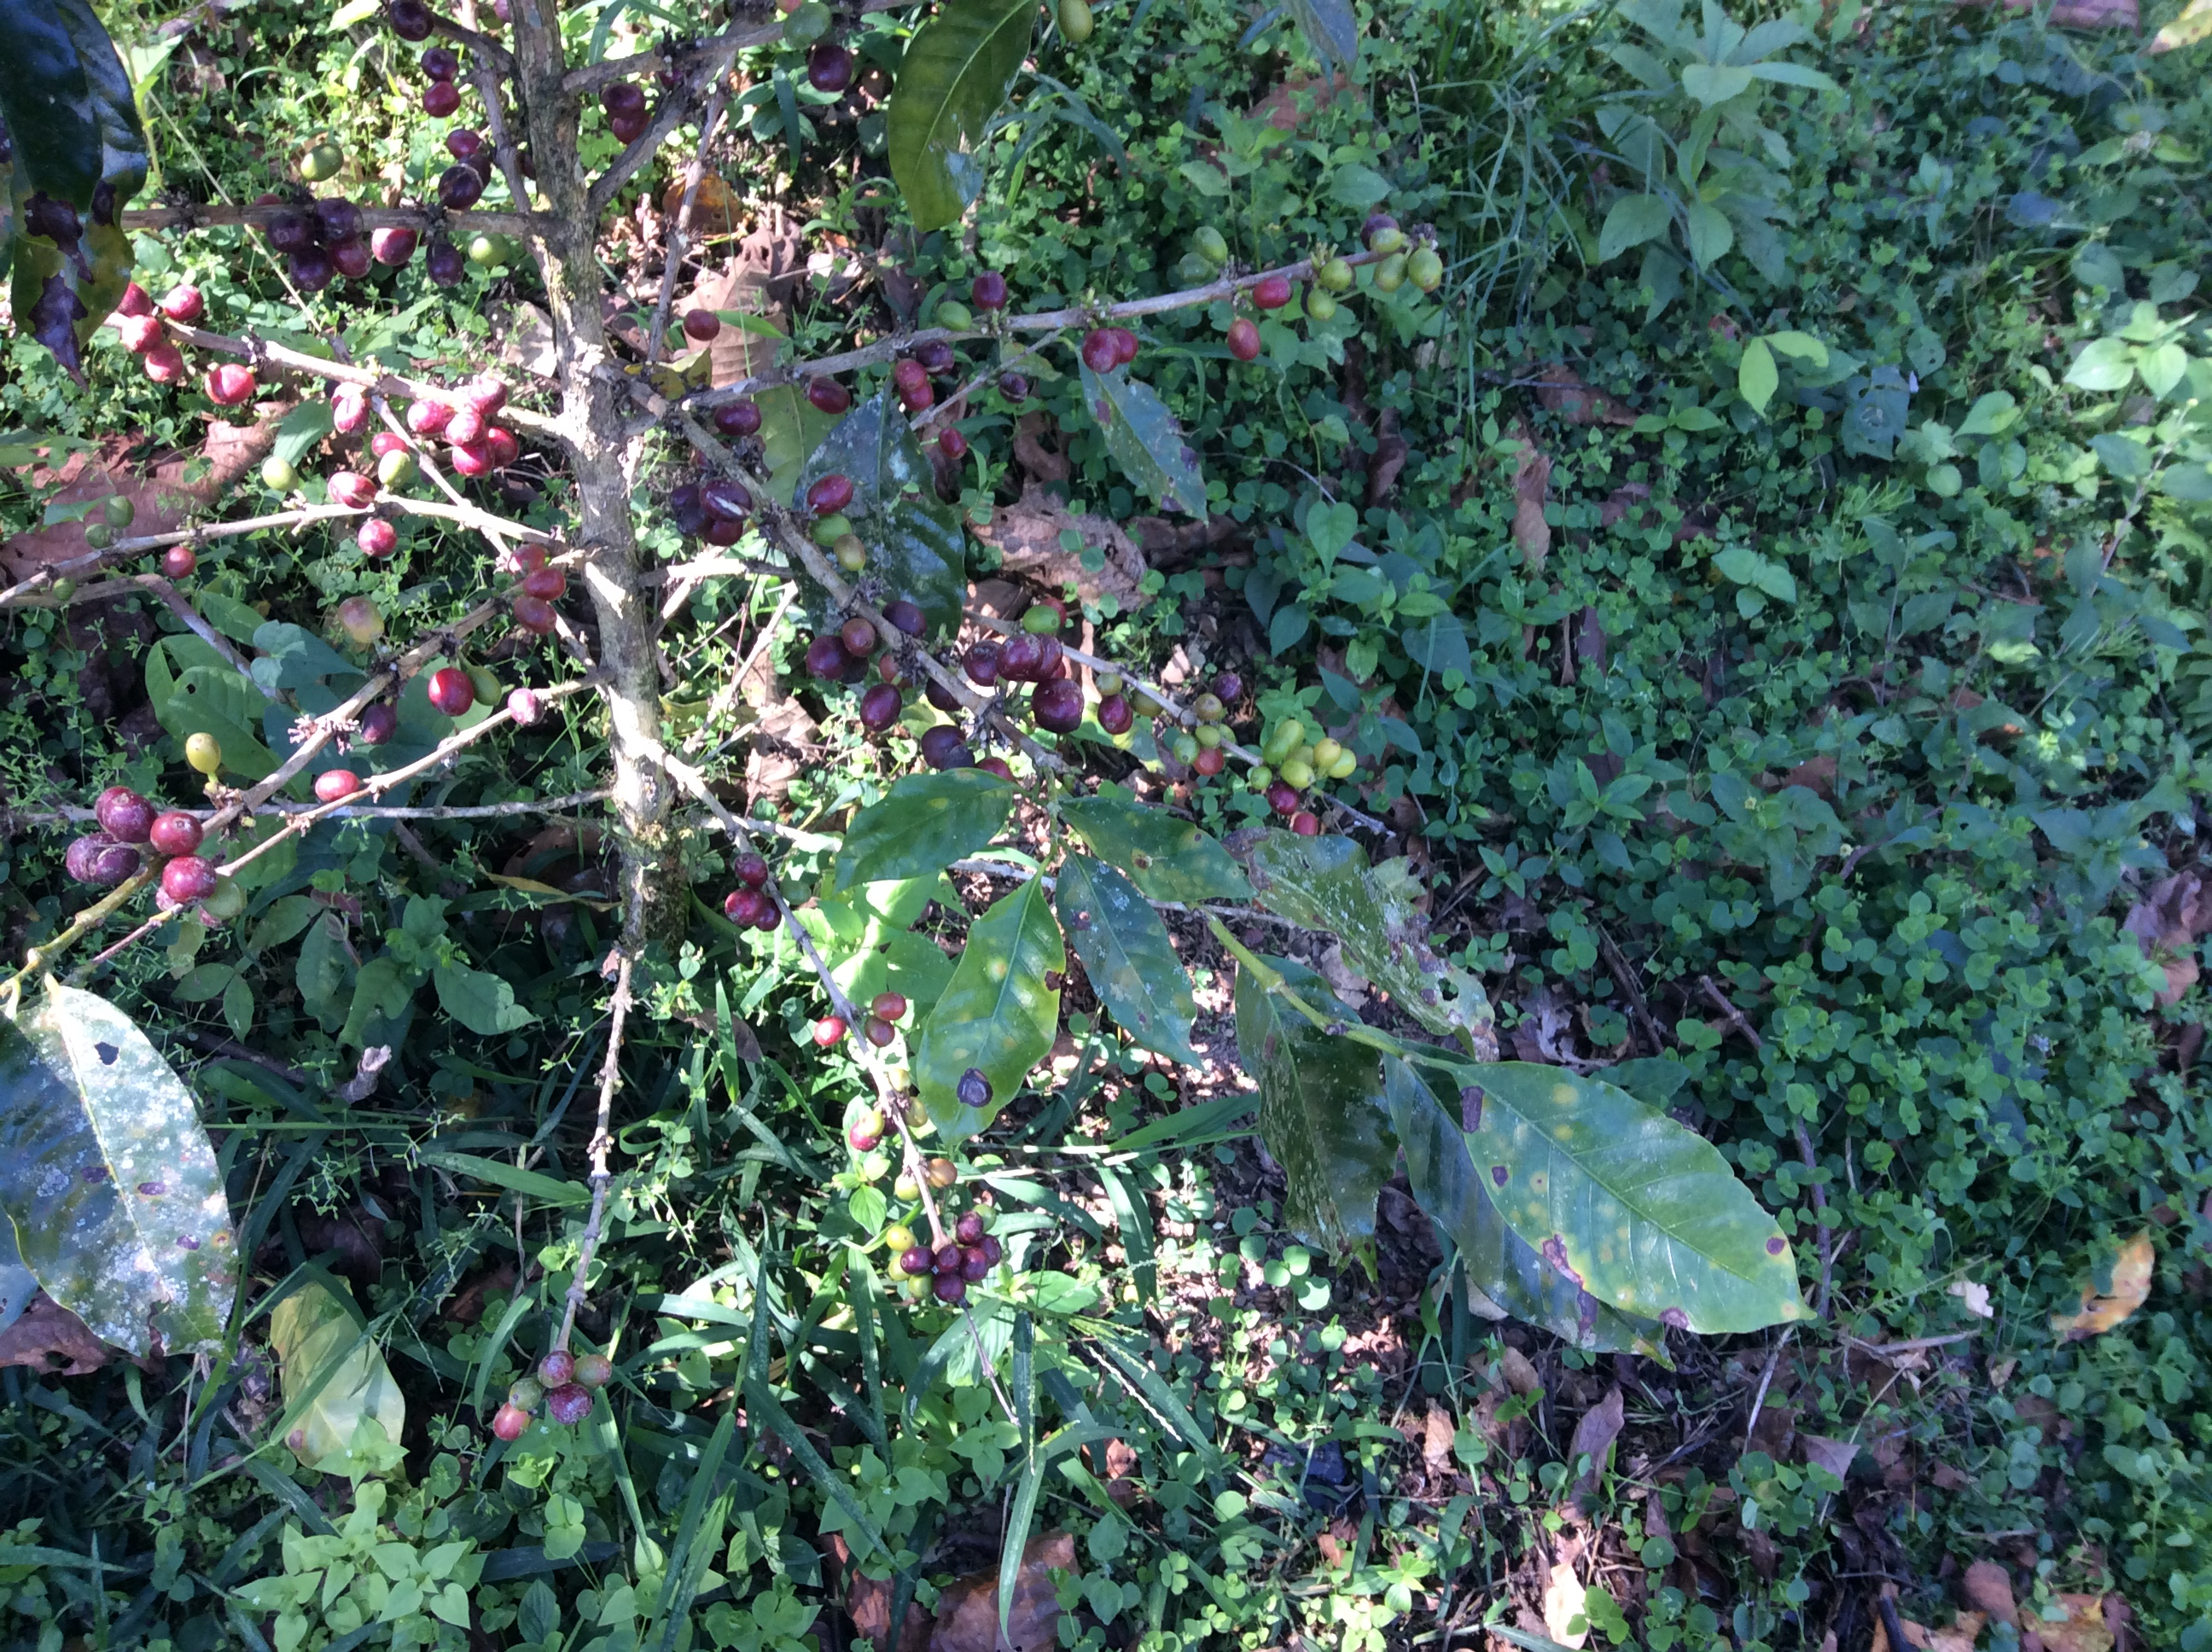
\includegraphics[width=0.99\linewidth]{IMG_0225.JPG}
\caption{Source image.}
\label{fig:data-color}
\end{figure} 

\subsection{Model}
Here a classification model is proposed through the function
$f_{\VECTOR{c}}:~\mathbb{R}^{3} \rightarrow \mathbb{R}$,
\begin{equation}
f_{\VECTOR{c}}(\VECTOR{x})=\frac{1}{1+e^{-h_{\VECTOR{c}}(\VECTOR{x})}},
\end{equation}
\begin{equation}
h_{\VECTOR{c}}(\VECTOR{x}) = c_1+c_2 x_1+c_3 x_2+c_4 x_3,
\end{equation}
where the column vector $\VECTOR{x}\in \mathbb{R}^{3}$ represents a pixel,
 with the $RGB$ additive color model,
 $\VECTOR{x}=[x_1,~ x_2,~ x_3]^{\transpose}\equiv [red,~ green,~ blue]^{\transpose}$
in the Fig. \ref{fig:data-color};
thus, the value $y=f_{\VECTOR{c}}(\VECTOR{x})$ indicates the state or label 
of sample $\VECTOR{x}$.
We consider that all color points  in the Fig. \ref{fig:data-color}
are separated principally in two sets (states); 
one set with color points that belong to a coffee seed,
with $y$ values close to $1$,
and another with everyone who doesn't belong, with $y$ values close to $0$.
The use of kernel function $h_{\VECTOR{c}}(\VECTOR{x})$ 
indicates that we assume that we can separate (approximately) 
these two sets by the hyper-plane $h_{\VECTOR{c}}(\VECTOR{x})=0$.

The function $f_{\VECTOR{c}}(\VECTOR{x})$, that is a modification of a sigmoid function,
has the characteristic that returns values between $0$ and $1$,
being that take a value $0.5$ when $h_{\VECTOR{c}}(\VECTOR{x})=0$;
%We consider that the function $f_{\VECTOR{c}}(\VECTOR{x})$ take values close to $1$
%when the color belong to a coffee seed, and the values close to $0$ when not;
%intermediate values indicates intermediate certainties;
remembering that the function $f_{\VECTOR{c}}(\VECTOR{x})$ only reaches $0$ and $1$ at $-\infty$ and $+\infty$,
respectively;
thus, our objective in the next sections will be found the column vector $\VECTOR{c}\in \mathbb{R}^{4}$,
where $\VECTOR{c}=[c_1,~ c_2,~ c_3,~ c_4]^{\transpose}$, that characterize the function $f_{\VECTOR{c}}(\VECTOR{x})$.

\subsection{Training}

To get the parameter vector $\VECTOR{c}=[c_1,~ c_2,~ c_3,~ c_4]^{\transpose}$
of function $f_{\VECTOR{c}}(\VECTOR{x})$, 
we need a set of training data like shown in the Fig. \ref{fig:data-trainning-bw},
\begin{figure}[h!]
\centering
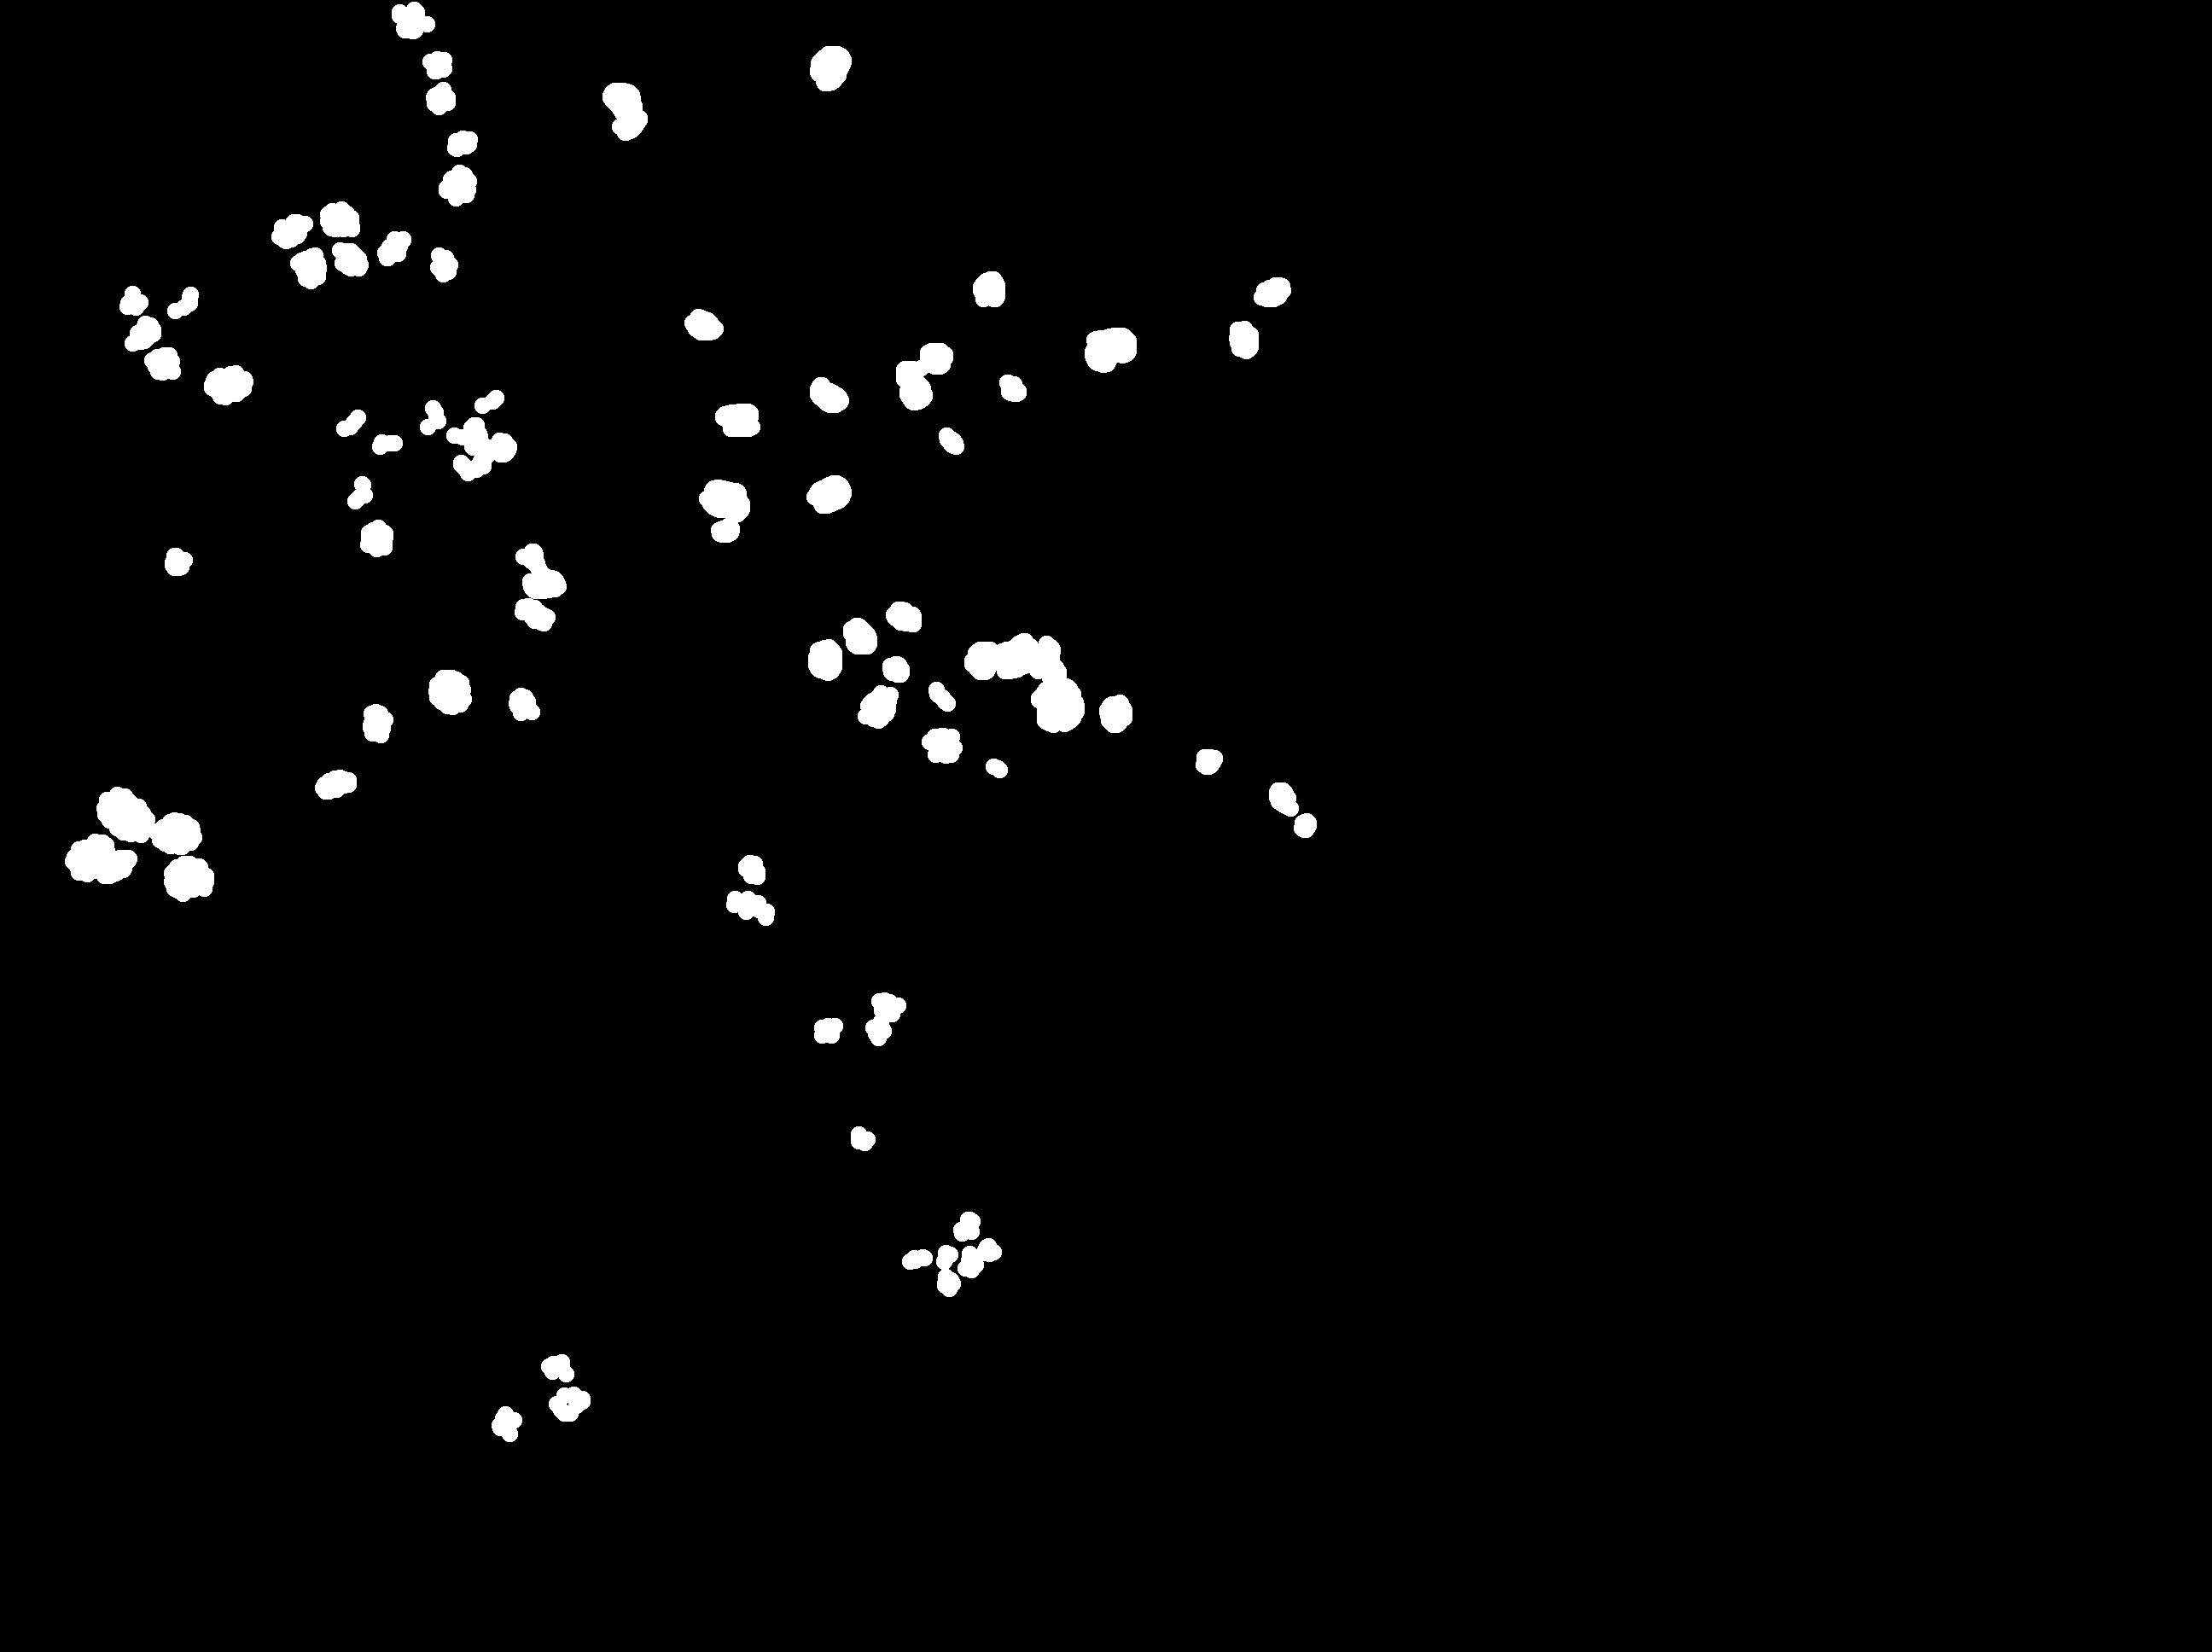
\includegraphics[width=0.99\linewidth]{IMG_0225-BW.png}
\caption{Training data.}
\label{fig:data-trainning-bw}
\end{figure} 
where the picture indicates with the white pixels, the approximate 
location\footnote{Manually painted.} of coffee seeds,
and the black pixels where not. 

Thus, using the pictures of Fig \ref{fig:data-color} and \ref{fig:data-trainning-bw},
we can training the model proposed in the function $f_{\VECTOR{c}}(\VECTOR{x})$
to get the vector $\VECTOR{c}=\VECTOR{\hat{c}}$
that optimizes the fit of training information.


